\chapter{Implementation}
This chapter deals with the details of the \emph{slicevis} package implementation. First, a brief overview of the user interface is given and then the internal methods and logic is laid out.

\begin{figure}[h]
	\centering
	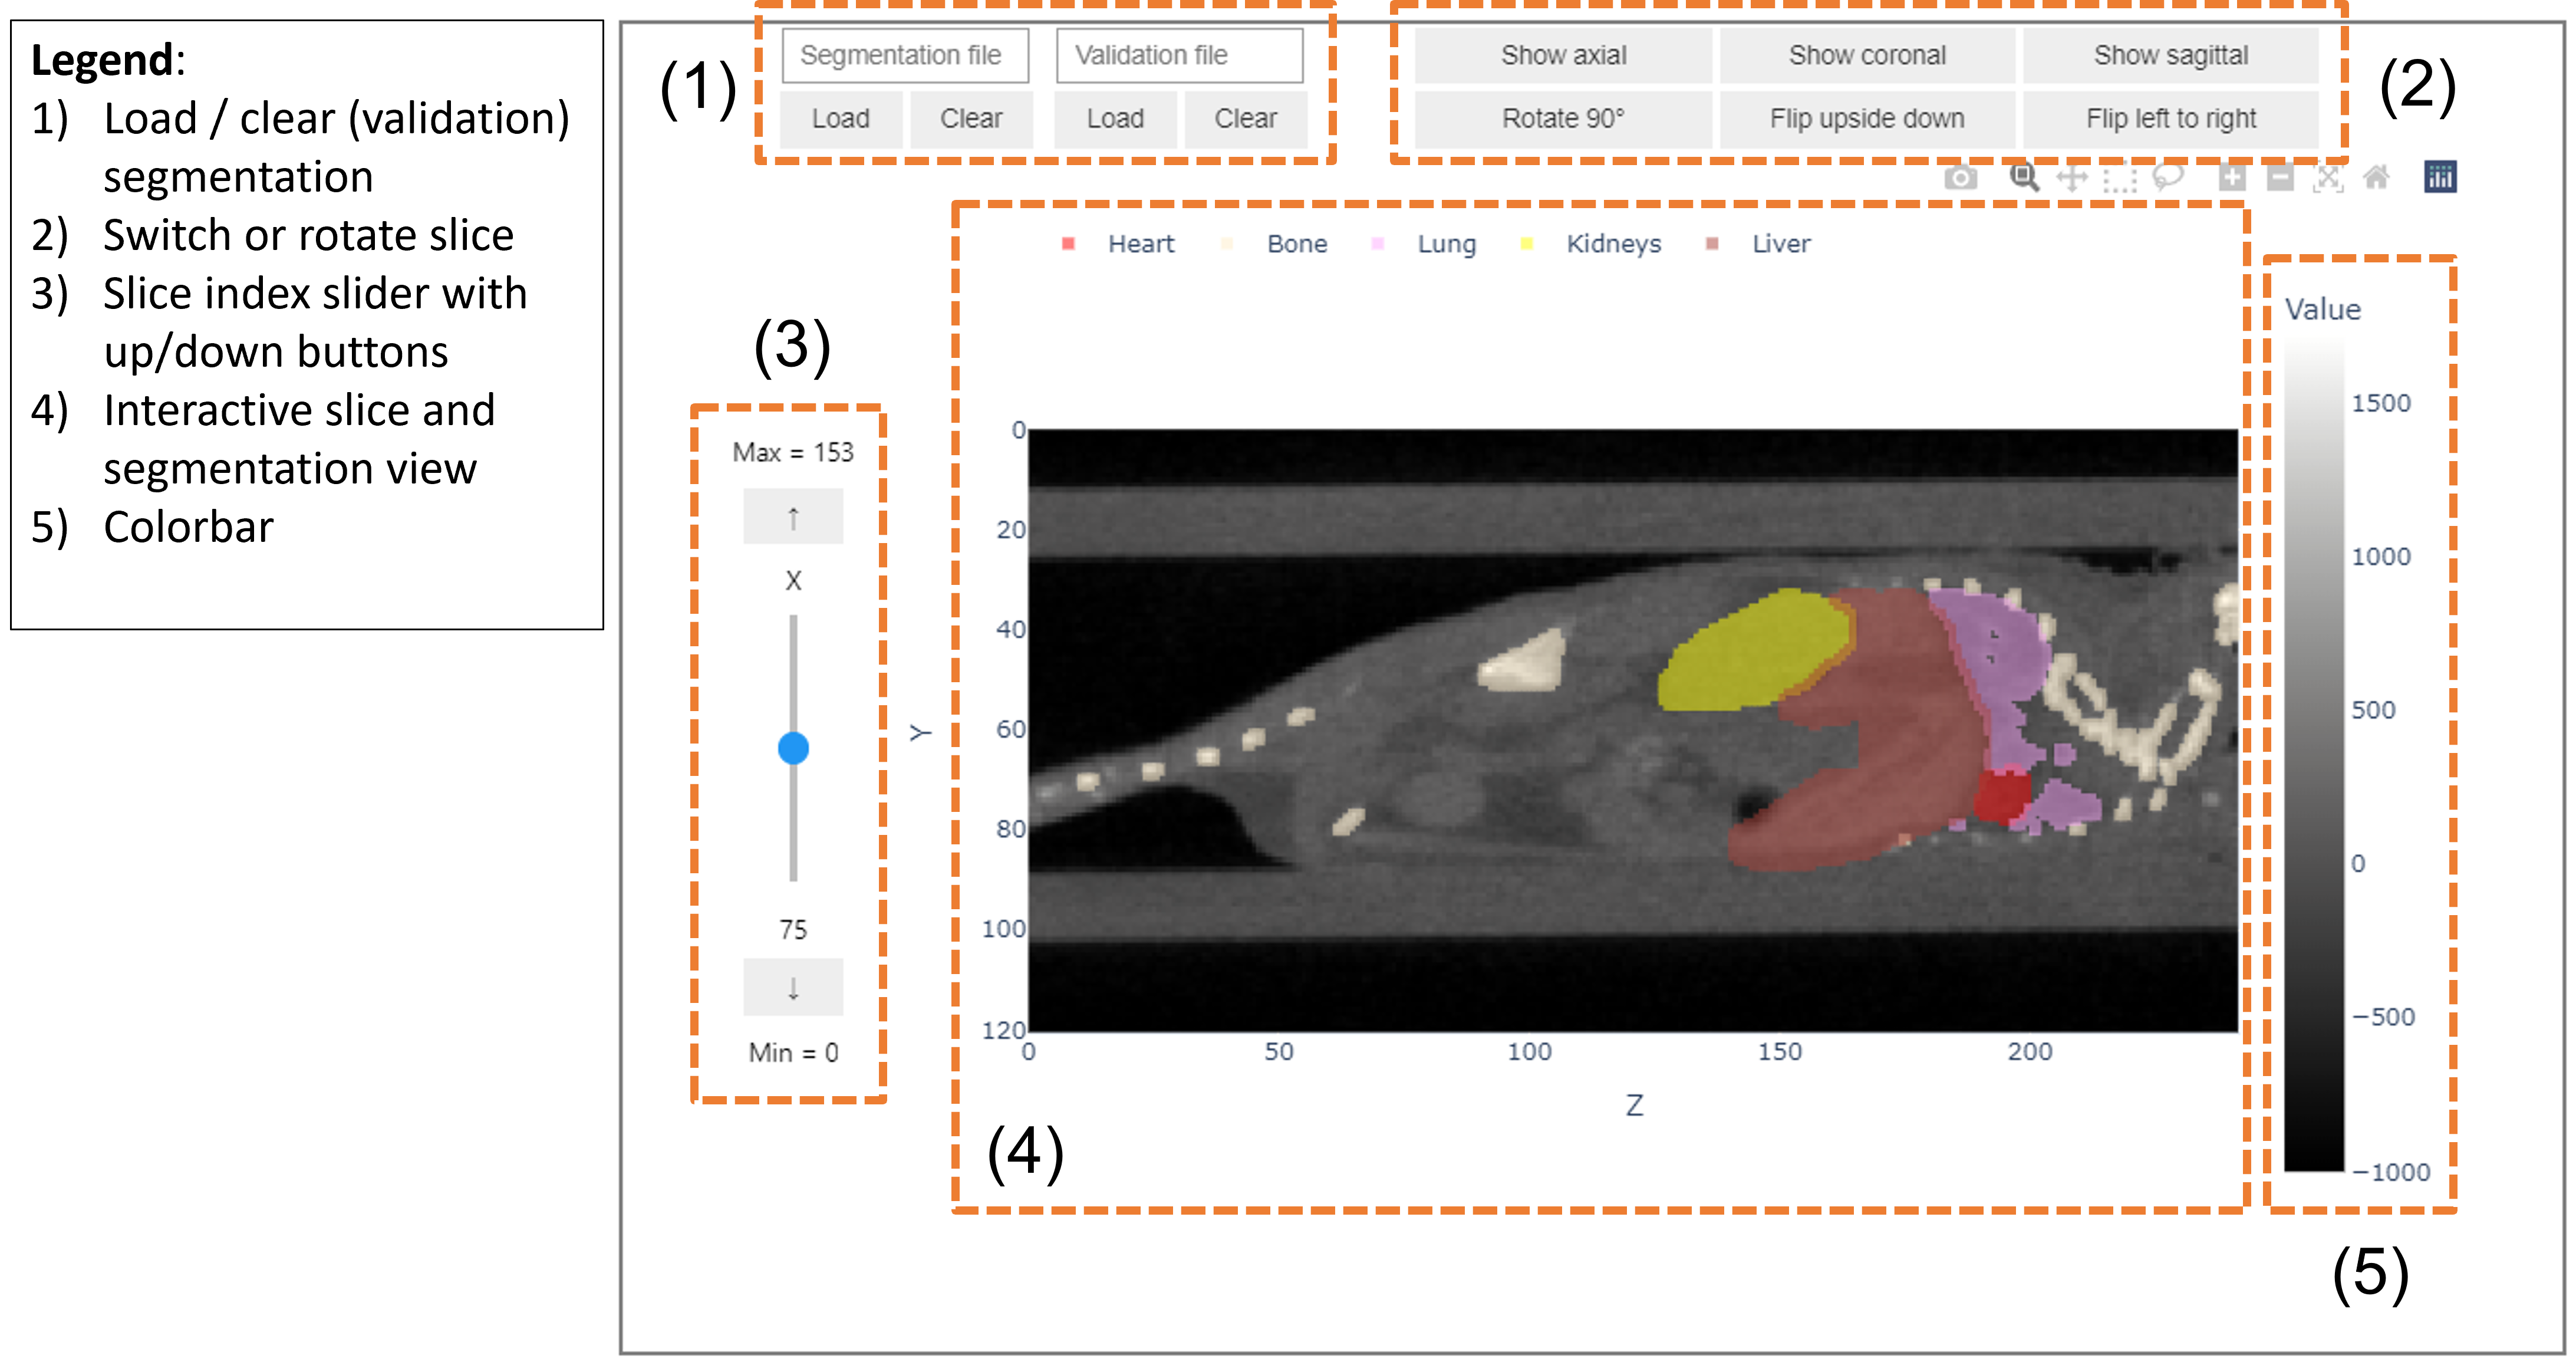
\includegraphics[width=\linewidth]{figures/GUI.png}
	\caption{The SliceWidget GUI, annotated.}
	\label{fig:gui}
\end{figure}

The main class of the package is \emph{SliceWidget}. It is implemented in \texttt{widget.py} and it is responsible for constructing the graphical user interface (GUI), rendering it in a Jupyter notebook and handling all user interactions. An annotated screenshot of the GUI is shown in \cref{fig:gui}. To build the interactive GUI, \emph{slicevis} relies on several other packages, namely \texttt{jupyter}, \texttt{ipywidgets}, and \texttt{plotly}. All buttons, sliders, text fields and the central updateable widget are available through \texttt{ipywidgets} \cite{ipywidget}. The 2D image, colorbar, and segmentation overlay are realized using the Plotly heatmap and scatter plot \cite{plotly}. Conveniently, the Plotly widgets provide buttons to zoom in, crop, and reset the view out of the box. To display the GUI, an instance of the \emph{SliceWidget} class must be created in a Jupyter cell \cite{jupyter}.

The \emph{SliceWidget} constructor expects a three-dimensional NumPy \texttt{ndarray} as input. There is also an optional debug mode which enables troubleshooting output and layout borders for developers. In the code, the \texttt{\_\_init\_\_} method adds all buttons, creates layouts, and connects function callbacks. Each widget in the GUI has at least one callback associated to it which performs some calculations and updates the slice view accordingly. \Cref{fig:callbacks} summarizes the connections between the buttons and the internal update method \texttt{\_update2D}.

\begin{figure}[h]
	\centering
	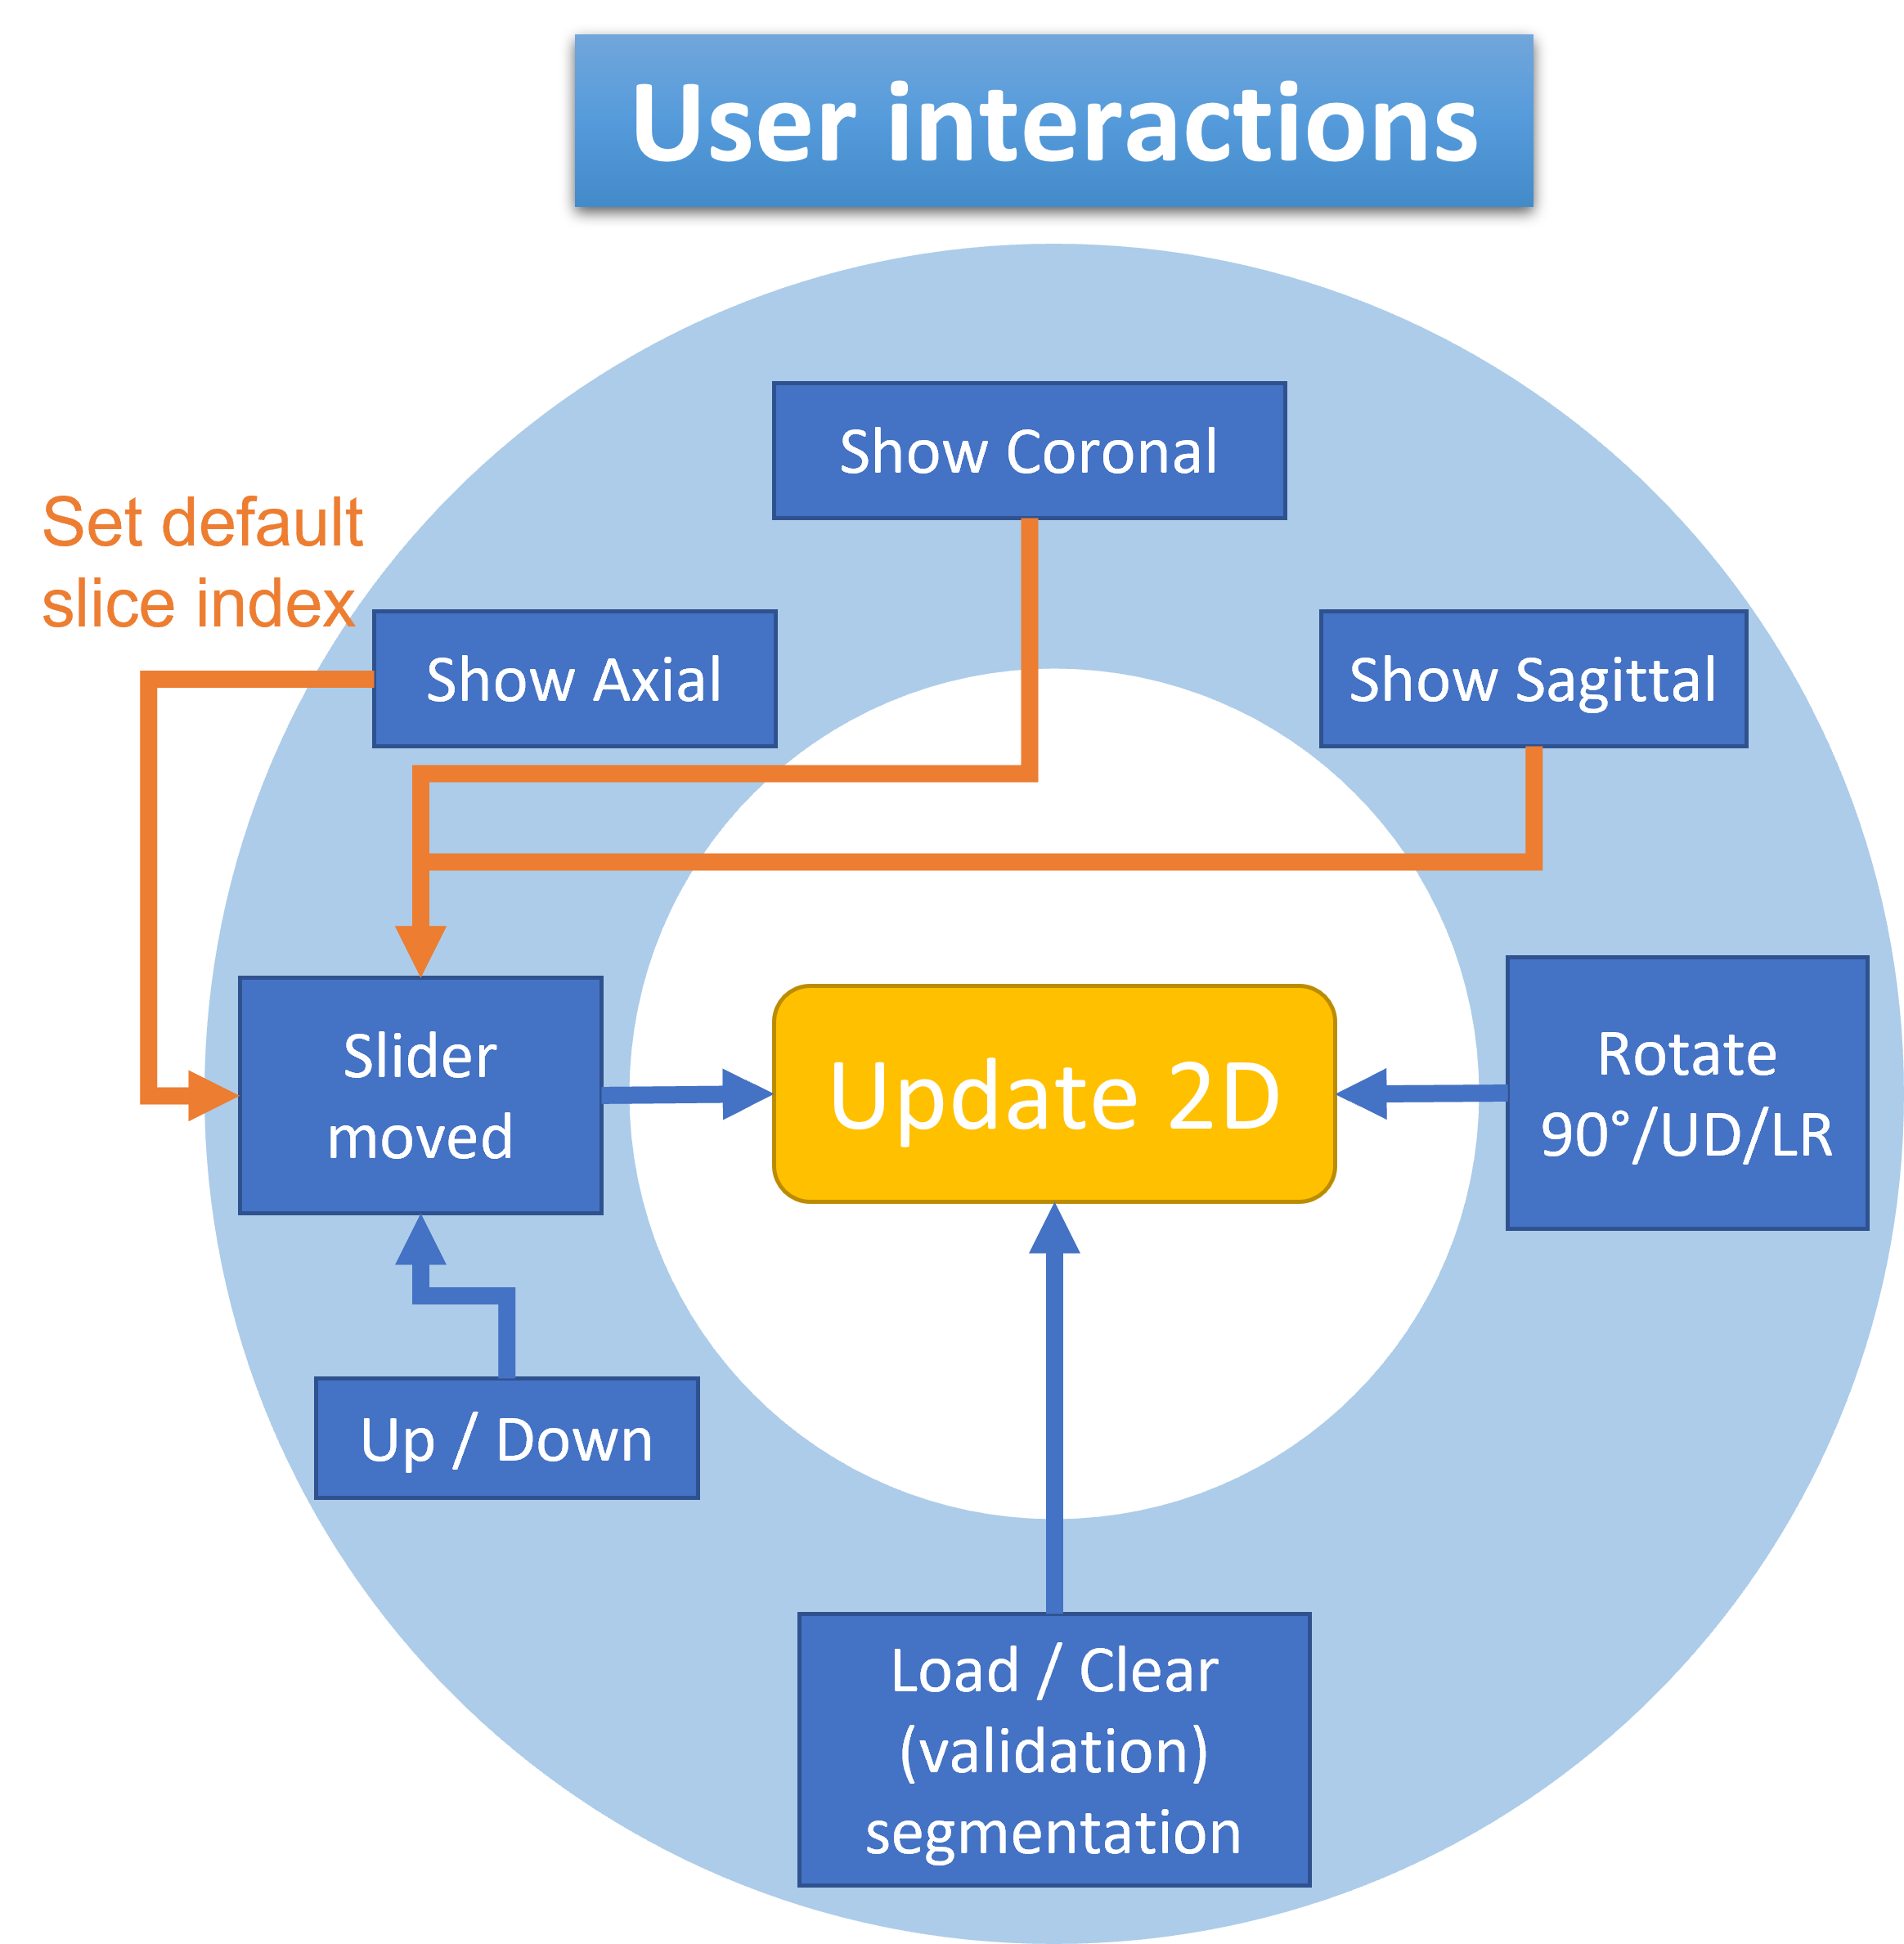
\includegraphics[height=.7\linewidth]{figures/call_graph.png}
	\caption{Call graph for interactive GUI update.}
	\label{fig:callbacks}
\end{figure}

The \texttt{\_update2D} method is the most important callback as it responsible for setting the 2D image to the correct slice each time the user interacts with the widget. \texttt{\_update2D} also paints the (up to) two segmentations as scatter plots on top of the image. As this method is called multiple times per second for smooth slicing, it must be reasonably efficient in its implementation. Updating the 2D image is as simple as indexing into the (possibly rotated) 3D image in the current axis where the index is given as input to the callback. The tricky part is painting the segmentations with their class names and colors on top. To find the pixels with coordinates $(x_i , y_i)$ of the class with index $j$ in the current slice, the \texttt{numpy} method \emph{nonzero(condition)} is used. As \emph{condition}, one can ask where \emph{self.seg2D} is equal to $j$. With the returned list of coordinate pairs, the class name, and its color, it is then possible to create a plotly scatter object and append it to a \emph{trace} list. This is repeated for each segmentation class. In the end, a \emph{batch\_update()} is called on the widget where the 2D image is swapped out and the trace list is added on top. By batching the updates to the widget, the render engine performs them all at once and flickering or delays are minimized. 

If both a segmentation and a validation segmentation have been loaded, the Dice score is automatically computed. A Dice score, also referred to as Sørensen–Dice coefficient \cite{dice}, is a measure of similarity between two segmentations. The score is always between zero and one, with one being a perfect match. It can be computed as follows:
\begin{equation}
	DICE(X, Y) =\frac{2|X \cap Y|}{|X|+|Y|}
	\label{eq:dice}
\end{equation}
where the operator $\cap$ is the intersection between $X$ and $Y$ and $|*|$ is the number of elements in the class. 

Lastly, it is worth pointing out that \emph{slicevis} supports a wide range of file formats. It has been only tested for NIfTIs (extension \texttt{.nii.gz}) and GFF (\texttt{.gff/.segff}) images so far but through the \texttt{nibabel} package also DICOMs are readable. The loading methods need to treat each file format separately in order to transform the data and metadata to a \emph{Image} instance (defined in \texttt{image.py}). GFF files are generally preferred for segmentations because the metadata already contains names and colors for the classes.

For more details, please refer to the documentation in the code.